\section{Introduction}
A language-model agent can ask the right question without receiving a reply from a person, issue a permission request without executing the associated tool, or trigger additional checking without correcting the underlying error. All three results may be scientifically valid. They answer different questions, however, from whether human oversight prevents harmful action in a deployed system. The distinction is especially consequential when a benchmark score is used to motivate an operational recommendation: the actor who supplied the answer, the state in which a decision occurred and the outcome actually measured determine what a reader may infer.

The same word can hide different experimental objects. An \emph{ask} event can be an episode-ending abstention, a question resolved by a stored answer, or a request submitted to a person in a live workflow. An \emph{approval} can be a binary classifier output, a simulated button action, or a consequential authorization granted by a human operator. A reduction in \emph{cost} may mean fewer generated questions, a model-judged attention score, lower elapsed laboratory time, or fewer measured minutes of active human work. Treating those measures as equivalent would erase the experimental conditions responsible for the result.

Prior scholarship has already established several of the distinctions at issue. Surveys of human--agent collaboration, abstention and human-in-the-loop design organize the relevant mechanisms \cite{ref1,ref3,ref4,ref5}. Nageshwaran and colleagues synthesize the validity of agent benchmarks \cite{ref2}; Yehudai and Mohammadi and colleagues survey evaluation methods and benchmark dimensions \cite{ref7,ref8}. Cao and colleagues map procedural integrity and quality in an explicit $\mathcal{F}^{*}$ framework \cite{ref9}, while Nguyen and colleagues distinguish the ability to intervene from normatively meaningful human control \cite{ref39}. Most directly, DelegationBench itself recommends separate reporting for candidate judgment, elicitation, permission resolution, constructed action, semantic correspondence and state update (Appendix J, Table 19) \cite{ref12}. An October 2026 narrative review in the target journal also maps AI-agent technical limitations to oversight, responsibility and incident-tracing problems \cite{ref48}; it does not reconstruct the particular missing-resolution labels or compare severity-conditioned observation across repositories. We do not claim to originate those reporting stages or to replace these broader reviews.

Our primary empirical question is narrower: when a released observational dataset records a resolution only for some agent--developer episodes, which numerical target is observed, which is only partially identified, and which cannot be inferred? We therefore reanalyze the pinned 16,118-episode release of Tang and colleagues \cite{ref35} using source-stratified, repository-matched and session-matched contrasts, then derive sharp missing-outcome bounds and an explicit sensitivity frontier for eventual post-pushback recovery. The cross-study checks that follow serve as interpretive context for the same target-definition problem; they are not a second systematic-review endpoint.

The central new descriptive contribution is an exact label-based test of whether the severity-related visibility difference persists not only across source streams and repositories but within the same recorded sessions. A second contribution shows how strong assumptions about the 14,614 unknown outcomes would have to be before the observed severity ordering could be translated into an eventual-recovery ordering. The release is based on episodes surfaced by developer pushback, not a census of unobserved agent failures. The original study reports limited expert annotation checks, with comparatively weaker severity-label agreement; our supplementary adversarial reclassification certificate shows that descriptive clustering stability is distinct from label-validity robustness. None of these analyses independently validates the severity labels, estimates a causal effect, or certifies agent safety. A compact machine-readable result file and deterministic replay script accompany the author-review package and export no third-party episode rows.

\section{Evidence basis and analytical approach}\label{sec:method}
\subsection{Primary empirical source and contextual source selection}
The primary empirical source is the public developer--agent misalignment annotation release accompanying Tang and colleagues \cite{ref35}. The frozen file contains 16,118 admitted misalignment episodes drawn from 20,574 original coding-agent sessions. The source defines an episode as a breakdown made visible through subsequent developer correction or pushback. Unnoticed failures, silent workarounds and sessions without visible pushback are outside this operational sampling frame. We analyze released labels exactly as assigned and pin the source by SHA-256 before admitting any result. The reanalysis scripts and aggregate-only replay certificate are publicly available at \url{https://github.com/shaikhamalkawi-ux/99llm-agent-oversight-reanalysis}; full numerical replay requires independently obtaining and hash-verifying the original authors' public annotation file. The source's codebook also shows why classification and resolution ascertainment may be linked: DS1 denotes effort/trust costs without an applied state change; DS2 requires an applied but readily reversible change; and RS1 requires explicit evidence of a fix. Because these assessments are drawn from the same conversation, trace observability can influence both the severity label and the apparent resolution rate. A positive within-session contrast therefore need not represent easier correction of objectively more severe failures. The source authors performed their own limited expert checks on the extraction and annotation pipeline: their public \href{https://arxiv.org/html/2605.29442v1}{May 2026 preprint v1}, Appendix A.2, Table 5, reports two-human exact agreement of 0.71 for \texttt{damage severity}, and model-to-adjudicated-label exact-match accuracy of 0.64, versus 0.92 and 0.96 for \texttt{resolution status}, on the 100-record annotation-check sample. These are source-reported, version-specific sample diagnostics, not an estimated DS1/DS2-specific confusion matrix or an accuracy claim for our reanalysis. We did not conduct a new manual severity-label validation, and the v1 diagnostic is not silently represented as a fresh test of the final conference edition.

A broader discovery register of 170 candidate source families was assembled earlier for contextual interpretation. AI-assisted title/abstract routing provisionally assigned 101 to possible primary-study work, 53 to contextual evidence and 16 to prior reviews. These are reading-queue categories rather than inclusion decisions: there is no exhaustive-search claim, registered protocol, PRISMA denominator or fieldwide sampling frame. Twelve detailed cases were selected retrospectively to illustrate contrasts in respondent, agent state, intervention timing, information budget, analysis unit or burden measure \cite{ref10,ref11,ref12,ref14,ref15,ref16,ref17,ref18,ref19,ref20,ref21,ref22}. A later four-case exercise and a seven-case challenge were likewise nonrandom. None is used to estimate prevalence in the literature or to validate the empirical DS1--DS2 result.

\subsection{Unit of analysis, source attribution and verification}
The unit of scrutiny is a \emph{source-specific claim about an experimental contrast}. Each claim is traced using eight descriptive fields: (A) source edition and locator; (B) runtime respondent; (C) decision and operational state; (D) timing relative to action; (E) comparator and information budget; (F) eligible unit, denominator and endpoint; (G) observed human effort or proxy; and (H) permitted inference. This record documents what was examined; it is not a validated scale, ranking or independent quality score. We separately identify (i) an original author's stated result, (ii) a value recomputed from displayed source evidence, (iii) a released-record recount, and (iv) an unresolved issue. A hypothetical overinterpretation by a reader is never attributed to the original authors without textual evidence.

Where an original table supplied counts, displayed fractions or model-level values, we recomputed only the permitted arithmetic. For released categorical data, we verified item identity, row counts and declared labels but did not rerun the source's collection or annotation models. We did not infer unobserved trial outcomes, invent missing user identifiers or reconstruct clustered $p$-values from aggregate tables. The evaluation combines original papers, publisher-version comparisons and selected author repositories; source access and any unclosed version gate are noted in the interpretation, not silently resolved by substituting a different edition. The supporting archive holds the bounded formulas, case-to-source links and version records. No third-party private user data are redistributed.

\subsection{Secondary observational analysis and dependence control}
For the released developer--agent annotation file, we first validate the declared SHA-256 source hash, distinct episode identifiers, resolution-status/resolver consistency, and the full data partition. The severity comparison is restricted to the two most prevalent labels, \texttt{DS1} (effort/trust) and \texttt{DS2} (easily reversible damage), using the original labels as assigned. The remaining 170 episodes with \texttt{DS0}, \texttt{DS3} or \texttt{DS4} are not silently reassigned or treated as successes. The binary descriptive outcome is \emph{visibly resolved} (\texttt{RS1}); \texttt{RS2} denotes \emph{unknown final outcome}, not failure.

We estimate raw visibility rates for each severity category and repeat the contrast in each original acquisition source (SpecStory and SWE). Because episodes are nested in repositories and repeated within sessions, we then perform two matched-cluster checks. First, among repositories containing both \texttt{DS1} and \texttt{DS2}, a repository is identified by (source, repository identifier); we compute the within-repository \texttt{DS2} minus \texttt{DS1} visible-resolution-rate difference and give each matched repository equal weight. We use 3,000 deterministic bootstrap resamples of whole repositories (seed 993718) as a descriptive resampling interval.

Second, we repeat the same calculation within recorded sessions, identified by (source, repository identifier, session identifier), retaining only sessions containing both severity labels. Each matched session receives equal weight. To avoid treating different sessions from one repository as independent resampling units, the preferred descriptive sensitivity interval resamples entire source--repository clusters and carries all eligible sessions in each sampled repository (3,000 replicates; seed 993720). For comparison we retain the original whole-session resampling interval (seed 993719), but do not treat it as a complete dependence correction. We also compute an equal-repository mean of within-session differences, a leave-one-repository-out range, and two explicitly post-hoc subset checks: episodes whose original extraction field \texttt{confidence} is \texttt{high}, and matched sessions with exactly one episode of each severity. The confidence field rates the support for an extracted episode, \emph{not} the quality of its damage-severity assignment. These are robustness descriptions, not multiple confirmatory hypothesis tests. Matching within a session absorbs factors constant at the recorded-session level, but it does not balance episode-level symptoms, causes, temporal order, task difficulty or annotation selection. None of the resampling intervals is a population confidence interval. No cases are reannotated, no model trajectories rerun and no causal severity parameter identified. Separately, we define an algebraic \emph{adversarial reclassification} check: keep each episode's observed RS1/RS2 outcome fixed while allowing its DS1/DS2 severity label to switch. We exhaustively enumerate the two outcome-concordant directions that can reduce the observed positive contrast, and find the fewest such flips needed to erase the sign. This is a worst-case source-label fragility certificate, not a data-derived measurement of misclassification, a new adjudication, or a validation of any particular corrected label.

\paragraph{Analytical tooling and assisted preparation.} All numerical findings are generated by deterministic Python scripts (standard library for source verification, recounting and resampling), with the conceptual figure generated by Matplotlib from the printed aggregate fractions. OpenAI ChatGPT was used substantively to assist literature selection, source comparisons, interpretation, code drafting and checking, and manuscript drafting and revision; it did not recruit participants or provide independently human-verified annotations. The authors must confirm the exact accessed product/version history and approve the results and this disclosure before submission.


\subsection{Evidence classes should not be collapsed}
Table~\ref{tab:objects} gives the main cross-setting distinction. A positive result in a lower-observability class is not a failed study; it is evidence about a narrower object. Stronger human-benefit or safety claims require a matching observed outcome and a suitable comparator.

\begin{table}[htbp]
\centering\small
\caption{Distinct experimental objects that can appear under the same intervention terminology. Examples illustrate measurement, not a hierarchy of study quality.}
\label{tab:objects}
\begin{tabularx}{\textwidth}{@{}p{0.21\textwidth}Y Y@{}}
\toprule
\textbf{Observed object} & \textbf{What can be learned} & \textbf{What it does not by itself establish}\\
\midrule
Offline choice or policy label \cite{ref12,ref13,ref42} & Recognition of the source-defined ask/call/allow category under a stated information budget. & Correct execution, real permission or downstream recovery.\\
Simulated reply during executable tasks \cite{ref14,ref23,ref41} & Agent behavior after information supplied by a model or stored response. & Human availability, effort or response quality in deployment.\\
Sandbox action trajectory \cite{ref12,ref24,ref32} & Tool choice, argument fidelity or scope compliance in a controlled environment. & Consequential external safety in an unmodeled service.\\
Human task or oversight session \cite{ref10,ref11,ref16,ref19} & Human behavior, checks and task outcomes within the tested protocol. & General workplace effectiveness without replication and matched assignment.\\
Deployment observation \cite{ref35,ref45} & Frequencies among selected recorded episodes and released labels. & Causal intervention benefit or unobserved eventual resolution.\\
\bottomrule
\end{tabularx}
\end{table}


\section{Results: recorded labels and identification limits}\label{sec:results}
\subsection{Recounting visible and unknown resolutions}
The pinned public annotation object released by Tang and colleagues permits a complete recount of its recorded labels \cite{ref35}. At the author-repository commit linked in the cited source, all 16,118 distinct episode IDs and the partition of 1,504 visibly resolved versus 14,614 with unobserved final resolution are reproducible. The visible subset classifies 45 episodes as agent self-correction, 1,376 as agent correction following developer pushback and 83 as developer takeover. The often-cited proportion \(1,376/1,504=91.49\%\) is \emph{conditional on visible resolution}; it is not the fraction of all identified episodes that eventually resolved after pushback. Most outcomes remain unobserved in the released labels, and the original authors already describe this selection limitation.

\subsection{Severity-conditioned visibility, matched clusters and uncertainty}\label{sec:newresult}
The two most prevalent original severity classes contain 15,948/16,118 recorded episodes. Table~\ref{tab:severity} reports direct counts and percentages from the pinned release. For \texttt{DS1}, 1,174/14,587 episodes (8.05\%) have a visible resolution; for \texttt{DS2}, 330/1,361 (24.25\%) do. Thus the pooled visible-resolution risk difference is 16.20 percentage points. It is present separately in the larger SpecStory source (23.04\% versus 7.67\%; +15.37 points) and in SWE (29.53\% versus 9.15\%; +20.38 points). These quantities describe whether the original released annotation includes a visible resolution, \emph{not} whether a case ever recovered or whether a developer's intervention caused recovery.

\begin{table}[htbp]
\centering\small
\caption{Visible resolution in the pinned 16,118-episode release by original severity label and data source. Only DS1 and DS2 appear in these contrasts. Percentages are episode-level; the repeated-episode dependence is addressed in separate matched-repository and matched-session analyses.}
\label{tab:severity}
\begin{tabularx}{\textwidth}{@{}lrrrrX@{}}
\toprule
Source & DS1 $n$ & DS1 RS1 & DS2 $n$ & DS2 RS1 & Visible-resolution difference (DS2--DS1) \\
\midrule
SpecStory & 10,861 & 833 (7.67\%) & 1,107 & 255 (23.04\%) & +15.37 percentage points \\
SWE & 3,726 & 341 (9.15\%) & 254 & 75 (29.53\%) & +20.38 percentage points \\
All records & 14,587 & 1,174 (8.05\%) & 1,361 & 330 (24.25\%) & +16.20 percentage points \\
\bottomrule
\end{tabularx}
\end{table}

Across 1,229 distinct source--repository keys represented in these two classes, 414 repositories contain at least one episode of each severity. Within this matched subset, the equal-repository mean \texttt{DS2}--\texttt{DS1} visibility difference is +15.87 percentage points; the deterministic 3,000-resample repository-cluster interval is +12.60 to +19.29 points. These repositories contain 12,643 of the 15,948 eligible episodes. For 163 of the 414 repositories the \texttt{DS2} visible-resolution proportion exceeds \texttt{DS1}, for 94 it is lower, and for 157 the proportions tie.

The stronger dependence check matches within the same recorded session. There are 853 sessions containing at least one \texttt{DS1} and one \texttt{DS2} episode, comprising 2,775 eligible episodes. In these sessions, 183/1,772 \texttt{DS1} episodes (10.33\%) and 240/1,003 \texttt{DS2} episodes (23.93\%) are visibly resolved. Giving every matched session equal weight yields a mean within-session difference of +13.96 percentage points; the 3,000-resample whole-session interval is +10.90 to +17.02 points. The session-specific difference is positive in 201 sessions, negative in 99 and tied in 553. Its equal-session mean remains positive in both source strata (SpecStory +12.52; SWE +20.46 points) and both recorded interaction modes (IDE +11.62; CLI +19.42 points). This removes explanations that depend only on factors constant within a session, but not explanations based on episode composition, ordering or selection. The result therefore strengthens a descriptive association rather than identifying a causal severity effect.

Because the 853 matched sessions belong to only 352 distinct source--repository clusters, repository-level resampling is the more appropriate dependence-sensitive summary. When all matched sessions from a selected repository are retained together, the same equal-session mean of +13.96 percentage points has a descriptive 2.5th--97.5th percentile interval of +10.72 to +17.30 points. The earlier resampling of whole sessions gave +10.90 to +17.02 points; we report it as a comparator rather than an independence-justified interval. The result is also positive when each of the 352 repositories contributes equally (+14.05 points; repository resampling interval +10.18 to +18.09 points). Deleting any one repository changes the equal-session mean only to between +13.56 and +14.36 points. These checks demonstrate stability of the recorded-label association to higher-level clustering and cluster weights, not external representativeness.

\begin{table}[htbp]
\centering\small
\caption{Repository-nested descriptive sensitivity of the within-session DS2--DS1 visible-resolution contrast. All values are percentage points, computed from the original labels. The percentile bands summarize resampling of observed clusters, not population confidence intervals. The final two rows are post-hoc subgroup checks, not confirmatory tests.}
\label{tab:nested}
\begin{tabularx}{\textwidth}{@{}YrrrY@{}}
\toprule
\textbf{Matched-session check} & \textbf{Sessions} & \textbf{Repositories} & \textbf{Mean difference} & \textbf{2.5--97.5 band} \\
\midrule
All paired sessions, equal-session weights & 853 & 352 & +13.96 & +10.72 to +17.30 \\
All paired sessions, equal-repository weights & 853 & 352 & +14.05 & +10.18 to +18.09 \\
Original extraction-confidence = high & 801 & 339 & +14.30 & +10.87 to +17.66 \\
Exactly one DS1 and one DS2 per session & 307 & 171 & +16.94 & +11.73 to +22.36 \\
\bottomrule
\end{tabularx}
\end{table}

The extraction-confidence and one-to-one restrictions were selected after inspecting available annotation fields and are exploratory. The original \texttt{confidence} field measures evidence support for an episode's extraction; neither restriction establishes correctness of its severity label. The one-to-one check removes multiplicity within included sessions but further reduces coverage; the original 853 matched sessions themselves contain only 2,775 of the 15,948 eligible DS1/DS2 episodes. The analysis should not imply that the matched subset represents the rest of the nonrandom released collection.


\subsection{Sensitivity to classification uncertainty}
The repository-nested resampling bands address dependence in the \emph{recorded labels}; they cannot address whether a reported DS2 episode should instead have been DS1 or vice versa. The source authors' 100-record validation check in arXiv v1 found materially weaker agreement on the severity axis than on the resolution-status axis (Section~\ref{sec:method}). This comparison does not furnish a joint error matrix, so we neither rescale the observed contrast by a guessed correction factor nor treat the sample error fraction as the corpus's DS1/DS2 error rate.

An exact worst-case label-perturbation check makes that remaining fragility concrete. Hold all 15,948 DS1/DS2 episodes' recorded RS1/RS2 outcomes fixed, and permit only a change in the \emph{severity} label within these two classes. We seek the minimum number of adversarial reclassifications making the pooled visibly-resolved rate for DS2 no greater than for DS1. Exactly \textbf{223} targeted flips suffice: reclassify 223 of the 330 original DS2/RS1 episodes as DS1/RS1, leaving the recorded outcomes untouched. The resulting rates are 107/1,138=9.40\% for DS2 and 1,397/14,810=9.43\% for DS1. Exhaustive integer enumeration of all directionally helpful combinations confirms that 222 or fewer flips cannot erase the pooled sign under this restricted two-class model. The threshold is 1.40\% of the 15,948 class-eligible labels; for SpecStory alone it is 170 records, and for SWE alone it is 55. The witness is \emph{adversarial and deliberately concentrated among visible DS2 outcomes}: it is not evidence that these labels are wrong, nor that this particular error pattern is likely. Thus the association is stable across observed clusters but not robust to unrestricted targeted label errors. The supplement records the exact integer search and assumptions.

For a severity group $g\in\{\mathrm{DS1},\mathrm{DS2}\}$, write $r_g$ for the observed fraction with resolver label RV2 and $u_g$ for the fraction with unknown final resolution. Without restrictions on missing outcomes, the eventual fraction $\theta_g$ and the group difference satisfy
\begin{equation}\label{eq:severity-bounds}
 r_g\leq \theta_g\leq r_g+u_g,\qquad
 r_{\mathrm{DS2}}-(r_{\mathrm{DS1}}+u_{\mathrm{DS1}})\leq \theta_{\mathrm{DS2}}-\theta_{\mathrm{DS1}} \leq (r_{\mathrm{DS2}}+u_{\mathrm{DS2}})-r_{\mathrm{DS1}}.
\end{equation}
These are sharp logical limits for the stated labels: every endpoint is attained by assigning appropriate outcomes to currently unknown cases. They do not make missing-outcome assumptions or identify causal effects.

The most important counter-result concerns \emph{eventual} resolution. Among DS1 there are 1,080 cases visibly marked \texttt{RV2} (agent resolution after pushback), and among DS2 there are 296. If every case without visible resolution may or may not eventually have resolved after pushback, the all-episode RV2 fraction lies between 7.40\% and 99.36\% for DS1, and between 21.75\% and 97.50\% for DS2. The logically permissible DS2-minus-DS1 eventual difference therefore spans about \emph{minus 77.61} to \emph{plus 90.10} percentage points. This bound contains large negative and positive values: the observed severity ordering of \emph{visibility} places no sign restriction on the eventual recovery contrast. Conditioning on visibly resolved outcomes creates still another target: 1,080/1,174 (91.99\%) in DS1 versus 296/330 (89.70\%) in DS2 are marked RV2.

A sensitivity frontier makes the missing-outcome requirement explicit. Let $q_1$ and $q_2$ denote the fractions of currently unknown DS1 and DS2 episodes, respectively, that would eventually receive resolver label RV2 if their terminal outcomes were observed. The implied DS2-minus-DS1 eventual difference is
\begin{equation}\label{eq:sensitivity}
\Delta(q_1,q_2)=\left(\frac{296}{1361}+\frac{1031}{1361}q_2\right)-\left(\frac{1080}{14587}+\frac{13413}{14587}q_1\right).
\end{equation}
The zero-difference frontier is $q_1=0.1560+0.8238q_2$. Thus, if no unknown DS2 case eventually resolved after pushback ($q_2=0$), the observed ordering would be erased once more than 15.60\% of unknown DS1 cases did; if $q_2=0.50$, the corresponding DS1 threshold is 56.79\%; and if $q_2=1$, it is 97.98\%. Under the special symmetry assumption $q_1=q_2=q$, the sign reverses only above $q=88.56\%$. These are tipping points under stated assumptions, not estimates of the unknown rates. Without such a restriction, the sign remains unidentified. None of these comparisons licenses calling unknown RS2 labels failures or treating the original labels as independently validated ground truth.

\begin{figure}[htbp]
\centering
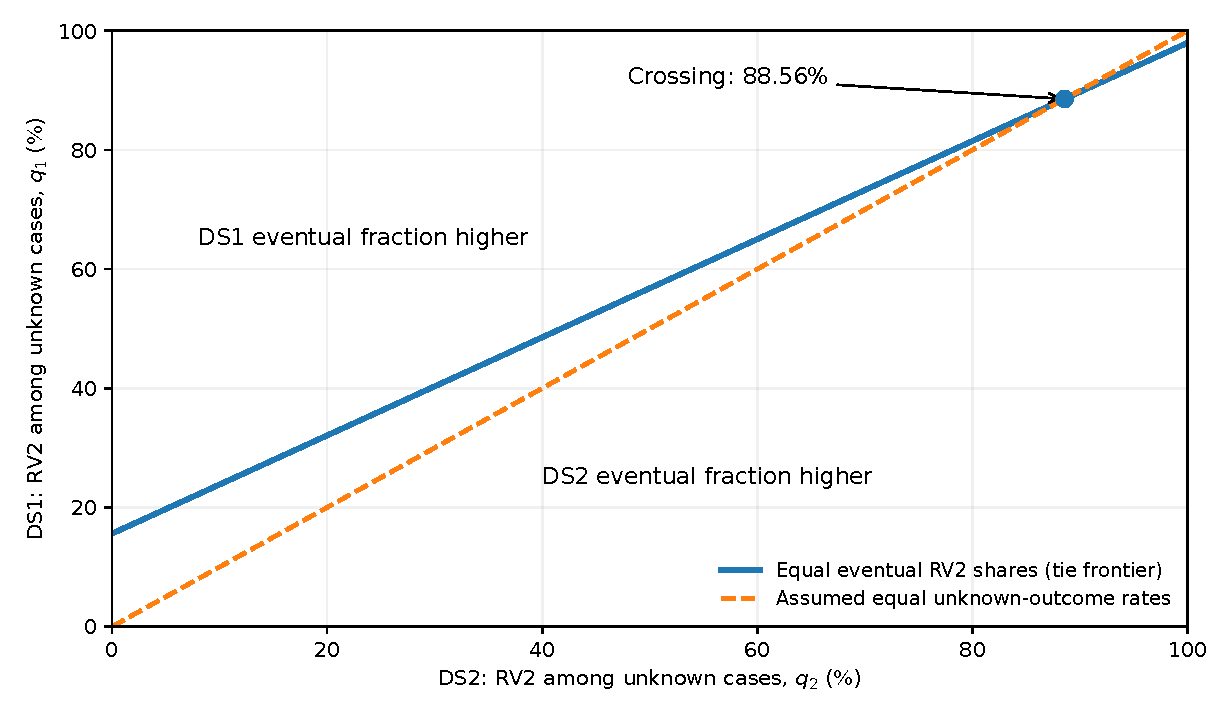
\includegraphics[width=0.84\textwidth]{figures/mr22_sensitivity_frontier.pdf}
\caption{Assumption-dependent sign boundary for the eventual DS2--DS1 after-pushback resolution contrast. The solid line gives values of $(q_2,q_1)$ at which the two fractions tie; points above it favor DS1 and below it favor DS2. The dashed line represents the unverified equal-unknown-rate assumption. The intersection is a sensitivity threshold, not a measured missing-outcome rate.}
\label{fig:frontier}
\end{figure}


\subsection{Partial identification of eventual post-pushback recovery}\label{sec:bounds}
The missing final-outcome labels give a precise example of why complete file reproducibility is not equivalent to identifying a population outcome. Let $N=16{,}118$ be the number of admitted episodes, $R=1{,}376$ the number with a \emph{visible} agent correction after developer pushback, and $U=14{,}614$ the number whose final resolution is unknown. If $R^{*}$ counts episodes eventually resolved by an agent after developer pushback, then the observed statuses alone imply
\begin{equation}\label{eq:bounds}
 \frac{R}{N}\;\leq\;\frac{R^{*}}{N}\;\leq\;\frac{R+U}{N},\qquad
 0.08537\;\leq\;\frac{R^{*}}{N}\;\leq\;0.99206.
\end{equation}
The bounds follow the standard partial-identification principle for missing outcomes: retain the observed classifications and allow each unknown outcome to fall on either side of the target \cite{ref47}. They do \emph{not} assume missingness at random or specify a predictive model. Thus the source's 91.49\% conditional figure remains correct for the 1,504 visibly resolved episodes, while neither the proposition that most \emph{all} episodes eventually recover after pushback nor its converse follows from the released resolution labels. The interval is a deterministic logical bound, not a confidence interval. A narrower empirical interval would require an outcome trace or a justified constraint on the 14,614 unknown cases; ordinary bootstrapping of the observed labels cannot provide that information.

This distinction is consequential for source comparisons. Studies reporting an intervention success rate conditional on an observed risk event address a well-defined selected population; studies with unobserved terminal outcomes cannot be pooled with them by renaming unknown as failure. The same issue occurs in observational oversight work when human intervention is preferentially triggered by difficult runs. It is a target-definition problem, not evidence that the original authors misstated their recorded counts.


\section{Contextual evidence: why intervention endpoints differ}\label{sec:context}
\subsection{Respondents, intervention points and agent states}\label{sec:actor}
\subsubsection{The runtime respondent matters}
A benchmark interface called \texttt{ask\_human} need not contact a person during an evaluated run. In HiL-Bench, agents encounter progressive software-engineering or SQL blockers, but replies are mediated by a frozen semantic matcher and stored blocker resolutions \cite{ref14}. Human experts contribute to constructing or checking tasks; they do not supply and time those runtime responses. The reported 300 tasks and 1,131 blockers therefore measure help-seeking in a simulated information environment. Learning to Ask and Ask-before-Plan similarly assess useful clarification with model-mediated or constructed users, although their designs and positive benchmark outcomes differ \cite{ref23,ref26}. Structured-uncertainty clarification methods report gains in source-defined answer coverage and questions asked with a simulated user; the original authors' uncertainty mechanism is their contribution, not evidence of observed human savings \cite{ref41}.

Human evidence may enter elsewhere. DelegationBench uses three people to label proposed actions, while its executable tests run in a sandbox; 149 of 156 labeled scenarios have a human majority decision, but those judgments are not live user authorization \cite{ref12}. Ask Less Ask Better uses professional ratings of selected prerecorded conversations to inform an attention-cost proxy while evaluating agents against simulated users at runtime \cite{ref20}. ReHAC combines a real-human HotpotQA arm with other simulated interactions, so its 14 annotators, 141 training questions and 1,937 trajectories must not be treated as the same number of individuals \cite{ref21}. Reporting simply \enquote{human-in-the-loop} without the task phase and actor would collapse these distinctions.

Direct simulator--human comparisons make the transport problem empirical rather than merely definitional. A study of user simulation for agentic tasks gathered 495 human dialogue traces over 165 tasks from 451 recruited people and compared them with multiple simulated respondents while holding the agent design fixed; its results show that simulator behavior and evaluation can differ from the human reference \cite{ref44}. That source independently establishes a simulator-fidelity concern and therefore limits any claim that the present review first discovered it. The narrower inference is that simulator suitability has to be established for the \emph{specific intervention outcome}, not assumed from the presence of human-created benchmark tasks.

\subsubsection{Asking, stopping and acting are different transitions}
The same event label can denote different transitions. Agentic Abstention treats a request for clarification as an episode-terminating abstain decision, whereas HiL-Bench allows a simulated answer to unblock execution and continue the task \cite{ref14,ref15}. An observed ask count in one study therefore cannot be pooled with a count of completed human-reply cycles from another. AgentAbstain and Designing for Doubt explore additional settings in which acting and withholding must be evaluated against feasibility and consequences rather than against a universal refusal target \cite{ref32,ref33}. A useful evaluation locates the \emph{earliest evidentially warranted} stop or question: ambiguity may already be visible at the request, whereas missing stock or a tool failure may only emerge after observation of the environment.

Authorization concerns a different transition. AuthGateBench tests an allow/block classification for a proposed action under different levels of policy information \cite{ref13}; AuthorizationBench executes policy-governed tool trajectories in mock services and observes the resulting state (286 tasks; 6,864 model runs) \cite{ref24}. This separation between judgment and state is also an explicit finding and recommended reporting stage of DelegationBench \cite{ref12}. A correct label, an authorized mock-service transition and actual live-human approval are three different endpoints. A pre-action sentinel can identify a proposed pause without establishing that a person reviewed or approved the action \cite{ref25}.

Action fidelity is itself an outcome distinct from a classifier label. In a released DelegationCheck action subset, the selected candidate tool appeared in 1,011 of 1,435 episodes, and 600 of those 1,011 matched both the selected tool and its arguments under a strict rule (59.35\%). This result describes a sandbox action-matching operator, not a probability that a user authorized or benefited from the resulting action \cite{ref12}. Whether asking or withholding improves this outcome depends on the tool's semantics, the policy and the comparator's information, none of which a standalone percentage can supply.

Finally, clarification can introduce an additional untrusted message. ASPI evaluates injection against agent states and response channels in simulated services, including an attacker-controlled reply to a clarification request \cite{ref31}. Its same-channel and cross-channel comparisons must be distinguished: changing the reply channel and the agent state at once does not isolate the effect of clarification itself. The implication is not that asking is generally unsafe; it is that a useful question and a secure answer channel are separate properties to evaluate.


\subsection{Human oversight: from checking to prevention and correction}\label{sec:human}
\subsubsection{More checks need not mean more repair}
Oversight has multiple stages: an action with possible adverse consequences occurs, the person notices or checks, an intervention is attempted, and the task either recovers or ends with an uncorrected outcome. These events cannot be collapsed into a single measure of \emph{human involvement}. In Looks Fine to Me, the published 71 seeded silent-defect episodes include 65 with some additional evaluation, yet only 28 finally corrected defects \cite{ref10}. The observed intervention may be generic, may fail to expose the problem, or may reveal an error that remains uncorrected. The source authors themselves separate behavioral from effective oversight; the additional arithmetic emphasizes that \(65/71\) and \(28/71\) measure different endpoints.

A controlled comparison of computer-use oversight strategies makes the denominator relationship explicit. Forty-eight participants each completed four sessions, giving 192 task sessions, not 192 people \cite{ref16}. Let $O$ denote a session with a problematic action, $I$ a successfully corrective human intervention among those sessions, and $F$ a final uncorrected failure. If the source's three mutually exclusive outcomes exhaust the session set---no occurrence, occurrence followed by correction, or occurrence without correction---then
\begin{equation}\label{eq:failure}
P(F)=P(O)\left[1-P(I\mid O)\right].
\end{equation}
The published rounded marginals reconstruct 138 sessions with a problematic occurrence, of which 29 included successful intervention and 109 ended uncorrected; the other 54 sessions had no such occurrence. Thus the displayed intervention rate is $29/138$ among exposed sessions, not $29/192$ among all sessions. The counts agree with the source's strategy and task-context margins. Equation~\ref{eq:failure} is an accounting identity under the stated partition, not a causal mediation analysis. The original paper reports a final-failure strategy contrast at $p=0.018$ but no corresponding difference in intervention success conditional on occurrence at $p=0.366$; its participant-clustered statistical model was not independently reconstructed from the available aggregate tables \cite{ref16}. Thus lower final failure need not mean users became better conditional error detectors; fewer adverse opportunities may be part of the explanation.

Observational intervention likewise introduces selection. Real human--agent web traces provide contextual evidence of interaction, but trajectories themselves are not independent users or a measured worker-hour saving \cite{ref27}. In Here Let Me Help, 30 participants contributed 360 web-agent sessions; 309 explicit stop events, 315 coded reasons and 322 type--reason incidences are legitimate but different denominators \cite{ref11}. Sessions in which users intervened had lower raw completion fractions than sessions without intervention, but users may have intervened precisely because a run was difficult. The raw association does not identify the effect of turning oversight on. Similarly, qualitative interviews and observed accounts of unintended GUI-agent outcomes document actual challenges and user strategies without estimating a randomized labor or safety effect \cite{ref29,ref30}.

\subsubsection{Time, attention and the autonomy of human judgment}
Human burden is not a single interchangeable unit. In TiCoder's interactive code-generation user study, the source reports better evaluated solution correctness and lower perceived workload under one workflow but no statistically established task-duration improvement; the setting is an adjacent coding-assistance task rather than a deployed autonomous tool agent \cite{ref18}. Cocoa's 16-person laboratory comparison allocates session time differently between inspection and co-execution, while its field phase reuses seven of the same participants \cite{ref19}. The session-time shares are not verified reductions in workforce hours. When Should Users Check? finds a 35.84-second difference between published mean elapsed times (264.70 vs 228.86 seconds) in controlled confirmation tasks with 48 participants; this is not an independently observed difference in active production labor \cite{ref17}.

Budgeted clarification studies make a related trade-off visible. Ask Less Ask Better reports 36--73\% lower \emph{judged} attentional cost while retaining 86--94\% of total task reward under specified question budgets. If the denominator is instead the reward \emph{increment attributable to asking}, the retained fractions are approximately 49\%, 71\% and 80\% across its three budgets \cite{ref20}. Neither statement is false solely because the other fraction is smaller; they are estimands with distinct baselines. The attention score is evaluated from sampled conversations, not stopwatch-measured burden from people answering during model rollouts. A deployed proactive agent similarly reports responses in 40.5\% of 22,594 observed on-call sessions after an analyst joined; the rate records delivery of proactive messages, not the number of incidents proven resolved or person-hours saved \cite{ref45}.

Human sign-off does not necessarily imply independent judgment, even when the reviewer is a professional. In a first-party industry experiment, agent preferences were randomized at four intermediate analytical decisions among 50 agent-using professionals; choices aligned with those assigned preferences 86\% of the time when pooled across decisions \cite{ref37}. The decision observations are repeated within people, and the intervention is the agent's randomized \emph{lean}, not random assignment to receive an agent. The report also finds a smaller final-recommendation contrast and cautions that the instructed preferences were deliberately strong. This is positive evidence of influence on expert choice in a bounded experimental setting, not evidence that every human approval is ineffective.

The studies observe different parts of human work: queries, rated attention, elapsed task time, intervention decisions and corrected outcomes. A fatigue-capacity analysis using stipulated reviewer behavior and agreement among three \emph{LLM personas} is informative about that model, but not observed fatigue or inter-human agreement \cite{ref46}. The original authors make that distinction; here it serves as a warning against replacing measured burden with a proxy.


\subsection{Source-table and release-edition checks}\label{sec:audit}
Published aggregate metrics can be reconstructed without rerunning an agent; the scope of that reconstruction must be reported just as carefully as the result. Table~\ref{tab:rechecks} distinguishes checks on displayed tables from a complete recount of released categorical labels. In particular, a source-internal table discrepancy is not evidence that the original experimental pipeline was wrong, whereas an incomplete outcome ascertainment problem can persist even when every released record has been counted.

\begin{table}[H]
\centering\small
\caption{Bounded reconstructions from published tables or publicly released labels. Counts reflect the study-specific eligible units; none estimates a fieldwide error rate.}
\label{tab:rechecks}
\begin{tabularx}{\textwidth}{@{}p{0.23\textwidth}p{0.33\textwidth}Y@{}}
\toprule
\textbf{Source and evidence} & \textbf{Independent check} & \textbf{Interpretive boundary}\\
\midrule
Dark Patterns, Table 3 \cite{ref22} & Across 16 categories: 10 strictly better under supervision, 4 tied, 2 worse; 14 are non-worse. & A non-worse count is not 14 strict improvements or statistical significance across categories.\\
Computer-use oversight, tables \cite{ref16} & Among 192 sessions: 54 no occurrence, 29 successful interventions and 109 uncorrected. & Recounts do not replicate participant-clustered inference or identify a causal pathway.\\
PULSE, seven printed score pairs \cite{ref36} & Ordinary unweighted Pearson $r=+0.302898$; table and prose present negative values ($-0.18$ and $-0.11$). & Printed-pair calculation does not reconstruct the unreported original regression or rating-to-arm experiment.\\
DRIFT-BENCH, publisher tables \cite{ref28} & One cell prints 46.33 without and 65.33 with clarification, but gain $+9.00$ rather than arithmetic $+19.00$. & The discrepancy is in printed table arithmetic, not a rerun of agent rollouts.\\
Developer--agent misalignment release \cite{ref35} & 16,118 labels: 1,504 visibly resolved, 14,614 unknown; eventual after-pushback share bounded by 8.54--99.21\%. & The 91.49\% reported among visible resolutions is conditional; the wide logical bounds do not validate the source classifier.\\
CAR-bench editions \cite{ref40} & Published task groups $100+90+50=240$; later competition groups $100+98+56=254$. & Different releases cannot be pooled as one task sample without record matching.\\
ClarifyBench, Table 2 \cite{ref41} & Printed total 716; explicit 241, ambiguous 213 and infeasible 198 sum to 652, leaving 64 unallocated by the printed categories. & This does not show why the 64 are unaccounted for or that the raw experiment omitted them.\\
\bottomrule
\end{tabularx}
\end{table}

\subsubsection{An operator or edition can change a source claim}
The source prose in Dark Patterns Meet GUI Agents describes fourteen of sixteen dark-pattern tasks as less susceptible under human supervision. Its printed avoidance-rate rows, however, yield ten strict increases, four ties and two decreases. Fourteen is the count of non-worse rows, not of strictly improved rows \cite{ref22}. Importantly, participants in the oversight arm watched prerecorded Operator trajectories, with pauses and confirmations simulated by the interviewer; the experiment does not test whether a live agent would have adapted after each intervention. This qualifies the interpretation of the direction count without erasing the observed supervised-condition benefits or the original study's qualitative analysis. Category directions alone do not supply within-participant significance tests.

For DRIFT-BENCH, the final ICML publisher edition and an earlier preprint contain related but noninterchangeable tables. The publisher's printed gain for one GPT-5.2 parameter-fault cell is ten percentage points lower than its displayed with-minus-without arithmetic \cite{ref28}. Its service-oriented appendix also contains both positive and negative clarification contrasts, so a blanket statement that clarification always helps or always hurts is unsupported. The original model-level and persona-specific inputs required to resolve the publisher's printed discrepancies are not available here. Reanalysis of a small, selected model roster cannot support population-level significance simply by adjusting multiple $p$-values; consequently we omit those exploratory significance calculations from the main scientific argument and retain them only in the internal evidence archive.

An especially clear operator distinction appears in CAR-bench. On the publisher's original 50 disambiguation tasks, the printed GPT-5 \(\mathrm{Pass@3}=68\%\) corresponds to 34 tasks with at least one success in three runs, while \(\mathrm{Pass}^{3}=36\%\) corresponds to 18 tasks successful in all three runs \cite{ref40}. These metrics answer different consistency questions. The publisher narrative also uses the label \(\mathrm{Pass@5}\) at one location for the value defined as \(\mathrm{Pass@3}\) in the source methods and table; this is a source-label conflict, not proof of additional undocumented trials. The later 254-task competition inventory is a different release from the 240-task paper and should be identified as such. In the published ClarifyBench table, domain-specific differences between the stated domain totals and the three enumerated query-type counts sum to 64; the source table alone cannot determine whether a fourth category, omitted rows or another reporting convention explains them \cite{ref41}. These checks illustrate why a numerator or printed label requires a versioned denominator before comparative interpretation.


\subsubsection{What a public feature release cannot reproduce}
PULSE combines observed developer feedback with prediction-assisted evaluation to compare software-agent designs and reports a reduction in confidence-interval width across its experiments \cite{ref36}. The seven published benchmark-versus-user-score pairs have an ordinary Pearson correlation of $+0.302898$ when recomputed from the printed values, whereas the published summary gives a negative sign. This sign difference is not explained by ordinary rounding of those displayed pairs. It nevertheless does not establish which transformation, weighting or unrounded records the authors used; the original calculation is a source-verification HOLD rather than a demonstrated error in their broader design comparison. The inspected public feature release contains 1,746 rated rows against 1,747 mentioned in the paper, but lacks the user-level treatment-arm joins and original fitted model inputs needed to rerun its four prediction-powered effect estimates. The reported original intervals and reduction are therefore attributed to the authors, not independently reproduced here.


\section{Discussion: interpretation and limitations}\label{sec:synthesis}
The reviewed experiments differ at the point where a benchmark outcome becomes an assertion about the agent or the person using it. The question is not whether every experiment should observe deployment. Rather, the reported claim should stay within the experiment's actor, state, counterfactual and endpoint. Table~\ref{tab:objects} separates the experimental objects, while Table~\ref{tab:rechecks} shows cases in which arithmetic or release identity alters the exact statement a reader can make. This synthesis does not produce a new composite benchmark score: assigning quality weights to different original study designs would replace identifiable source conditions with a judgment that has not been externally validated.

Three implications follow for interpreting and designing studies. \emph{First}, when comparing policies for asking or abstaining, experiments should hold the available policy, task information, tools and question budget constant, or identify those differences explicitly. A tool-call bias measured as an offline next-action selection cannot be treated as a field safety endpoint merely because an activation-steering intervention improves the correct no-call class \cite{ref42}. Likewise, controlled shared-control mazes with four human operators and repeated trials can reveal adaptive allocation under route advantage but not a general benefit to all workplace users \cite{ref43}.

\emph{Second}, intervention studies should report the transition they change, rather than using a generic notion of success. For a risky action, distinct outcomes include prevention of occurrence, detection conditional on occurrence, successful correction, rollback and uncorrected final harm. The occurrence--intervention--failure decomposition in Equation~\ref{eq:failure} displays the necessary denominators, but, without suitable assignment and clustered data, does not identify a causal mechanism behind a final-failure contrast. For clarification, the relevant sequence begins with the first missing fact and continues through useful reply and correct post-reply action. Broader agent evaluations already identify cost, robustness and execution context as distinct axes \cite{ref2,ref7,ref34}; future interventions should specify where in that sequence their evidence ends.

\emph{Third}, claims of human benefit should involve a human-benefit measurement. Lab timing, perceived workload, simulated-user satisfaction, model-judged attentional cost and real user work minutes provide different information. Observational proactive responses or human approvals are not substitute measures of corrected incidents or genuinely independent expert judgment. The distinction is not an argument for discarding simulated benchmarks: they can efficiently and reproducibly test mechanics, provided their generalizability is evaluated rather than presumed \cite{ref44,ref46}. Further scrutiny of evaluation validity is also consistent with existing critiques of outcome-focused agent benchmarks and with procedural approaches that already require explicit source-to-measurement links \cite{ref8,ref9}.

\subsection{Interpretive and methodological limits}
This is a secondary observational reanalysis with purposively selected cross-study source checks, not a systematic review of the field. The 170-family register cannot support fieldwide percentages; its screening statuses are provisional; the twelve detailed cases and later challenge sets are not independent random draws. They are retained only to show why respondent, state, denominator and endpoint distinctions matter when interpreting the primary 16,118-episode result. The A--H trace has not been compared with a human-adjudicated reference standard or tested for sensitivity, specificity or superiority over existing review practices. We do not claim a second human coder or inter-human agreement coefficient.

The empirical checks also have unequal reproducibility depth. Original tables permit exact arithmetic without identifying hidden rounding, task matching, treatment assignments or the authors' clustered statistical models. The complete annotation file permits exact label counts, source stratification and matched-cluster calculations without validating how the labels were originally constructed or determining outcomes never observed. The primary empirical finding is therefore a source-stratified, repository-matched and session-matched descriptive association in the original severity and resolution labels. Matching by session removes only differences in factors constant across episodes within that recorded session. Repository-nested resampling accounts for the higher clustering level in a descriptive way but does not remove episode-level confounding by cause, symptom, timing or annotation mechanisms. The underlying labels have not been independently revalidated by us; unlike a dataset without any quality audit, the source itself reports a limited expert adjudication check, with weaker severity-axis performance in the explicitly cited arXiv v1 edition. Moreover, the source codebook uses the same visible interaction to establish applied damage and explicit correction; this measurement coupling offers a plausible noncausal explanation for part of the visibility contrast. Neither session matching nor clustering separates that common ascertainment process. Its small, imbalanced reference sample cannot estimate error specifically between DS1 and DS2. Our exact 223-label adversarial certificate further demonstrates that the sign of the pooled visibility contrast is conditional on a potentially fragile severity assignment; repository clustering does not address this vulnerability. Moreover, because a case is included only after visible developer pushback, the recorded corpus is neither all agent errors nor a probability sample.

The closest priority constraint is substantive rather than terminological. General evaluation-validity and procedure-aware surveys already provide audit structures \cite{ref2,ref9}, and DelegationBench directly recommends a staged judgment-to-state reporting protocol \cite{ref12}. Original research on user simulators and fatigue modeling likewise establishes respondent- and workload-related limits \cite{ref44,ref46}. Our contribution is the bounded reconstruction and attribution of particular published contrasts, not the first invention of those boundaries. Demonstrating that this approach improves decisions relative to existing review standards would require a separate comparative study.


\section{Conclusion}
An agent-intervention statistic becomes interpretable only when its actor, decision state, analysis unit, denominator and endpoint are retained. In the pinned 16,118-episode coding-agent release, the DS2--DS1 visible-resolution contrast is large at the episode level and remains positive across both acquisition sources, matched repositories and, more stringently, matched sessions. The same data do not identify the sign of the eventual post-pushback recovery difference because most terminal outcomes are unknown. The sensitivity frontier shows exactly which assumptions about those unknown outcomes would be required to preserve or reverse the observed ordering; under equal unknown-case recovery rates, reversal occurs only above 88.56\%, but that equality is itself unobserved. The source's 91.49\% after-pushback figure remains valid for visibly resolved episodes and cannot establish an all-episode recovery majority. The observed contrast also fails a worst-case severity-label robustness test with 223 targeted relabelings, a mathematical sensitivity witness rather than evidence of actual annotation mistakes. These results strengthen a reproducible descriptive reanalysis without turning severity into a causal exposure or treating published annotation checks as our independent validation. Generalized agent safety, saved human labor and superiority over previous audit frameworks remain untested.

